% !TeX program = xelatex
\documentclass{article}
\usepackage{iclr2026_conference,times}

\usepackage{graphicx}
\usepackage{float}
\usepackage{amssymb}
\usepackage{amsmath}
\usepackage{fontspec}
\setmainfont{Tinos}[
  Path=fonts/,
  Extension=.ttf,
  UprightFont=Tinos-Regular,
  BoldFont=Tinos-Bold,
  ItalicFont=Tinos-Italic,
  BoldItalicFont=Tinos-BoldItalic,
]
\usepackage{booktabs}
\usepackage{array}
\usepackage{tabularx}
\usepackage{enumitem}
\usepackage{pifont}
\usepackage{xcolor}
\usepackage{hyperref}
\usepackage{url}
\usepackage{tikz}
\usetikzlibrary{arrows.meta,positioning,calc}

\emergencystretch=1.2em
\setlist{nosep,leftmargin=*}
\setlength{\textfloatsep}{10pt plus 2pt minus 2pt}
\setlength{\dbltextfloatsep}{6pt plus 2pt minus 2pt}
\setlength{\dblfloatsep}{6pt plus 2pt minus 2pt}
\setlength{\abovecaptionskip}{4pt}
\setlength{\belowcaptionskip}{0pt}
% The ICLR style enables \flushbottom. With non-breakable [H] result tables,
% that stretches section/table glue into conspicuous holes. Keep the normal
% inter-block spacing and leave any unavoidable remainder at the page foot.
\raggedbottom

\definecolor{auditblue}{HTML}{0077BB}
\definecolor{auditteal}{HTML}{009988}
\definecolor{auditorange}{HTML}{EE7733}

% Tinos does not expose an OpenType small-caps face. Scale the interior capitals
% explicitly so the M and P remain full-size in the paper-title lockup.
\newcommand{\MuralPresenterLogo}{\mbox{M\raisebox{0.08ex}{\scalebox{0.78}{URAL}}P\raisebox{0.08ex}{\scalebox{0.78}{RESENTER}}}}
\newcommand{\sys}{MuralPresenter}
\newcommand{\fullsys}{\MuralPresenterLogo}
\newcommand{\bench}{ThreadBench}
\hyphenation{ThreadBench}
\newcommand{\tbd}[1]{\textcolor{auditorange}{\textsc{[TBD-#1]}}}
% Preserve unique placeholder IDs in source while keeping result tables readable.
\newcommand{\resulttbd}[1]{\textcolor{auditorange}{\textsc{TBD}}}
\newcommand{\pilot}[1]{\textcolor{auditteal}{\textsc{#1}}}

\title{\fullsys: Multi-Agent Unified\\
Reasoning and Authoring for Long-Horizon\\
Presentations}

\author{Anonymous authors}

%\iclrfinalcopy
\begin{document}

\maketitle

% Generated mechanically from the reviewed Markdown source.
% Controller edits should be made in both source and LaTeX when material.

\begin{abstract}

A presentation slide can look correct in isolation yet contradict the deck: a term defined early is silently redefined later, a visual encoding reverses meaning, or a numerical premise is consumed but never established. Such failures arise because authoring decisions persist across stages and pages while execution contexts do not. The missing design variable is responsibility granularity: which pages must share an owner. \textbf{MuralPresenter} externalizes persistent deck state and delegates production to dependency-aligned, non-overlapping slide groups, each jointly authored, rendered, and revised by one Group Agent. Its four-phase workflow grounds content, freezes a deck-wide plan, produces independent groups in parallel, and closes residual relations through whole-deck review. A companion synthesis pipeline enriches three query tracks with Style profiles and task-conditioned long-horizon dependencies, then compiles them into checklists for trajectory filtering. We train MuralPresenter-9B on 1,000 quality-controlled trajectories and MuralPresenter-27B on a larger heterogeneous cohort, and introduce \textbf{ThreadBench} to score intermediate process evidence separately from final artifact quality. On PresentBench, MuralPresenter-9B and MuralPresenter-27B obtain \resulttbd{[TBD:ABS\_M9\_PB]} and \resulttbd{[TBD:ABS\_M27\_PB]} Overall; on ThreadBench they reach \resulttbd{[TBD:ABS\_M9\_THREAD]} and \resulttbd{[TBD:ABS\_M27\_THREAD]} Final. Controlled ablations attribute \resulttbd{[TBD:ABS\_ABLATION\_SUMMARY]} to dependency-aligned responsibility and render-grounded trajectory supervision. Together, the results show how explicit ownership and auditable handoffs support long-horizon presentation authoring.

\end{abstract}

\section{Introduction}

A presentation is a persistent decision object. Authors fix terminology, choose color encodings, set numerical premises, and establish narrative arcs before production begins. These decisions are consumed across distant slides and revisited across versions \citep{maheshwari-etal-2024-presentations,zheng2025pptagent,xu-etal-2025-pregenie}. When consumption fails, a page appears valid in isolation while contradicting the whole: current evaluations report omitted requirements, unsupported claims, numerical errors, and broken cross-slide consistency \citep{chen2026presentbench}.

This persistence creates a dilemma. A single Agent retains unified context but accumulates execution artifacts into a growing history that weakens its use of earlier decisions \citep{sun2025contextfolding}. Stage- or page-level decomposition isolates subtasks but fragments responsibility; whether it helps depends on task structure, information sharing, and validation placement—not on Agent count \citep{kim2025scalingagents}. Neither extreme asks: which pages should jointly own a dependency?

\textbf{MuralPresenter} answers with the \textbf{slide group}. The Orchestrator partitions every page into complete, non-overlapping groups by narrative purpose, design affinity, and cross-slide dependency. One Group Agent generates, inspects, and revises all pages in its group; independent groups run in parallel; whole-deck Review backstops relations that span groups. Persistent state is externalized so each stage reads a projection rather than raw history; deterministic parsing, downloading, rendering, and building remain tools. Figure~\ref{fig:page-topologies} contrasts this topology with sequential and per-slide alternatives. HTML serves as the authoring source, with image, PDF, and PPTX conversion treated as delivery boundaries.

\begin{figure*}[t]
\centering
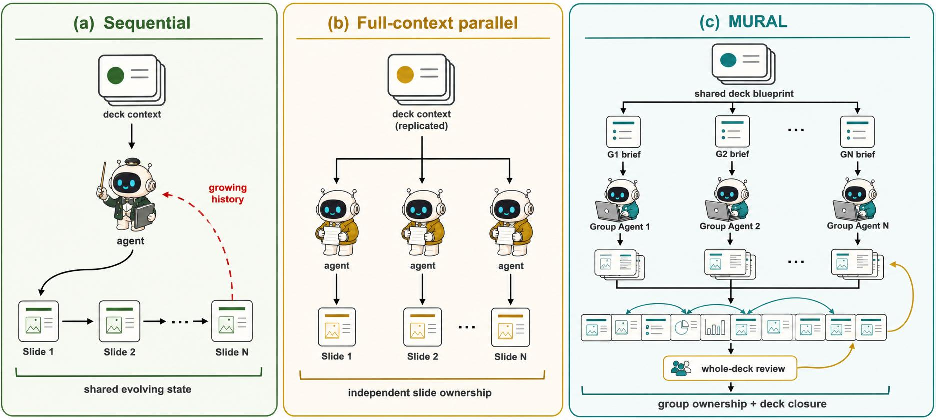
\includegraphics[width=0.90\textwidth]{figures/fig1_page_topologies.pdf}
\caption{\textbf{Three page-production topologies and their responsibility boundaries.}
Sequential generation keeps one growing history; full-context parallel gives each worker one slide from copied
deck context. \sys{} externalizes shared state, compiles dependency-aligned groups, and makes one Group Agent
jointly generate and inspect each group. Within-group relations therefore share an owner, while whole-deck
Review handles the remaining cross-group relations.}
\label{fig:page-topologies}
\end{figure*}


The same dependencies that define slide groups govern training. Three query tracks feed a shared enrichment layer that injects Style, constructs task-conditioned long-horizon dependencies, and compiles them into a QC checklist; candidate trajectories are filtered against that checklist. We train MuralPresenter-9B on a controlled 1K trajectory corpus and MuralPresenter-27B on six heterogeneous historical batches under quality control and reweighting (§4). \textbf{ThreadBench} (Tracing Handoffs, Requirements, and Execution Across Deck Generation) evaluates process--artifact consistency, including cross-page semantic consistency in its Final Deck rubric; PresentBench and SlidesGen-Bench complement it with general quality and DECKBench with multi-turn revision. Our contributions are:

\begin{enumerate}
\item \textbf{A full-lifecycle, skill-based authoring framework} with an explicit boundary between deterministic tools and isolated Agent contexts.
\item \textbf{A dependency-aligned responsibility topology} in which one Group Agent jointly owns related pages, and edits replay only at the necessary scope.
\item \textbf{A controllable synthesis pipeline and two trained models:} MuralPresenter-9B uses 1,000 post-QC trajectories from the three-track construction, while MuralPresenter-27B uses six quality-controlled historical batches.
\item \textbf{ThreadBench}, a process-aware, artifact-grounded evaluation of intermediate handoffs and final deck quality, paired with general-generation and multi-turn-editing benchmarks.
\end{enumerate}

The remainder of the paper reviews related work (§2), presents the authoring system and data pipeline (§§3–4), defines ThreadBench and the evaluation protocol (§§5–6), and closes with a traceable case study, validity boundaries, and conclusions (§§7–8).

\section{Related Work}

\textbf{Presentation generation.} Content-selection methods address what belongs on each slide \citep{bandyopadhyay-etal-2024-enhancing-presentation,maheshwari-etal-2024-presentations}; Agent systems add deck planning \citep{zheng2025pptagent}, render-grounded review \citep{xu-etal-2025-pregenie}, specialized roles \citep{xie2026slidebot}, iterative visual refinement \citep{zheng2026deeppresenter}, slide–script coordination and delivery \citep{yang2026deepslide}, and design–code decoupling \citep{cui2026designfirst}. Slide–script coordination and delivery support are prior art; MuralPresenter's distinction is slide-group ownership of cross-slide source-to-target relations.

\textbf{Long-horizon state and Agent granularity.} Growing history impairs the use of earlier information before the context window is exhausted \citep{sun2025contextfolding}; externalizing verified state and launching fresh contexts can stabilize long trajectories \citep{ma2026longhorizonharness}. Because decomposition gains depend on task structure and information flow \citep{kim2025scalingagents}, MuralPresenter aligns group boundaries with dependency structure rather than pipeline stages or page indices.

\textbf{Agentic data and refinement.} Full interaction traces preserve planning decisions and tool use \citep{zeng2023agenttuning,chen2024agentflan}, while iterative feedback teaches diagnosis and repair \citep{madaan2023selfrefine}. MuralPresenter instead accepts trajectories against machine-checkable dependencies injected before rollout; controlled ablations test whether inspect–diagnose–patch traces transfer to editing.

\textbf{Benchmarks.} PresentBench evaluates material-grounded generation \citep{chen2026presentbench}; SlidesGen-Bench covers Content, Aesthetics, and static Editability \citep{yang2026slidesgenbench}; DECKBench studies generation and multi-turn editing \citep{jang2026deckbench}. PPTArena and PPT-Eval probe compound or PowerPoint-native edits \citep{ofengenden2025pptarena,gandhi2026ppteval}, and LH-Bench rates process and output with Skill-grounded rubrics \citep{gupta2026lhbench}. ThreadBench complements final-only evaluation by scoring case-specific Research, Planning, Image, and Slide-production evidence separately from Knowledge, Deck, and Page quality.

% Generated mechanically from the reviewed Markdown source.
% Controller edits should be made in both source and LaTeX when material.

\section{MuralPresenter}

Figure~\ref{fig:release-workflow} gives the system overview. MuralPresenter first externalizes the task and deck state, then assigns only independently acceptable work to fresh Agent contexts, binds dependent pages to shared Group Agents, and closes residual relations through render-grounded review. Sections 3.1--3.3 respectively formalize the task and state projection, specify role boundaries, and define grouping, visual critique, and scope-based revision.

\subsection{The Long-Horizon Presentation Task}

We formulate presentation authoring as an interactive agentic task. Given a user request \(q\), optional attachments \(\mathcal{M}\), a language \(\ell\), and a target length \(N\), the system operates with tool library \(\mathcal{T}\) and persistent state \(\mathcal{S}\), producing a deck \(D=(s_1,\ldots,s_N)\) together with per-slide notes and renders.

The generation process is a multi-step trajectory \(\tau\) decomposed into four phases: \[
\tau \;=\; \tau^{\mathrm{ground}} \circ \tau^{\mathrm{plan}} \circ \tau^{\mathrm{gen}} \circ \tau^{\mathrm{review}},
\] corresponding to content grounding, deck-wide planning, grouped generation, and whole-deck review. A downstream phase does not begin until its dependencies are ready in \(\mathcal{S}\); the generation phase further decomposes into disjoint page-group trajectories \(\tau^{\mathrm{gen}}=\{\tau^{G_1},\ldots,\tau^{G_m}\}\) running in parallel, where \(\{G_1,\ldots,G_m\}\) partitions \(\{1,\ldots,N\}\) (§3.3).

State externalization grounds this phase ordering. Each accepted artifact \(d\) enters \(\mathcal{S}\) with a fixed producing phase and owner role. A role \(r\) reads only its declared projection: \[
\pi_r(\mathcal{S}) \;\triangleq\; \{d \in \mathcal{S} \mid d \text{ is in } r\text{'s declared read-set}\},
\] and model-generated writes target only its declared write-set. In implementation, \(\mathcal{S}\) corresponds to the deck's persistent state directory, each Skill's role card declares \(\pi_r\), and the delegation topology enforces which artifacts a fresh context receives; deterministic scripts may still derive or update shared state on behalf of any role. The projection thus formalizes the delegation contract—what each role is responsible for reading and producing—rather than hard filesystem isolation.

The task is \emph{long-horizon}: an opening thesis must resolve at the end, and terms or visual encodings defined early must be reused throughout. We write such a relation as a cross-slide dependency \(g_k=(a_k,T_k,\Phi_k)\): source page \(a_k\) establishes a decision, target set \(T_k\) consumes it, and predicate \(\Phi_k\) tests whether the relation holds. Deck-level consistency is then characterized by whether these dependencies close (§5); MuralPresenter's design turns on which roles bear joint responsibility for cross-slide dependencies at which lifecycle boundary.

\subsection{Skill-Driven Multi-Agent Collaboration}

MuralPresenter expresses responsibilities as pluggable Skills that specify when a role is triggered, which projection of \(\mathcal{S}\) it reads, what it produces, and the handback criterion. A separate Agent is opened only when work can be delivered and accepted independently; otherwise the Orchestrator proceeds with tools.

\textbf{Orchestrator.} Interprets user intent, coordinates grounding, plans the deck, delegates production, and accepts results—but does not search images, write pages, or judge pixels. Deterministic operations (parsing, downloading, rendering, building) are invoked directly as tools. Per-slide spoken scripts are fixed during planning and deterministically compiled into a unified speech artifact before production. Group Agents implement only the frozen visible-content contract without rewriting scripts. After render-grounded whole-deck Review, a final deterministic pass re-synchronizes the speech artifact.

\textbf{Material \& Research.} Material parses attachments into structured summaries; Research verifies only external facts that would change a conclusion. Both consolidate outputs into citable grounded knowledge. Neither role appears when no attachment and no external fact is at stake.

\textbf{Image.} Opened only when a page plan genuinely needs photographs or generated pictures; it isolates retrieval, generation, candidate comparison, and pixel inspection from the global trajectory.

\textbf{Group Agent.} Each Group Agent owns one page group and, along a single bounded trajectory \(\tau^{G_j}\), jointly generates and inspects all pages in that group (§3.3), maintaining within-group relations without negotiating with other groups. Independent groups run in parallel.

\textbf{Review.} After generation converges, a Review role that took no part in generation performs an independent whole-deck inspection in an isolated context, avoiding self-assessment bias (§3.3). The build tool then packages the final artifact and validates consistency. Figure~\ref{fig:release-workflow} connects these ownership boundaries to the complete authoring, revision, and delivery lifecycle.

\begin{figure*}[t]
\centering
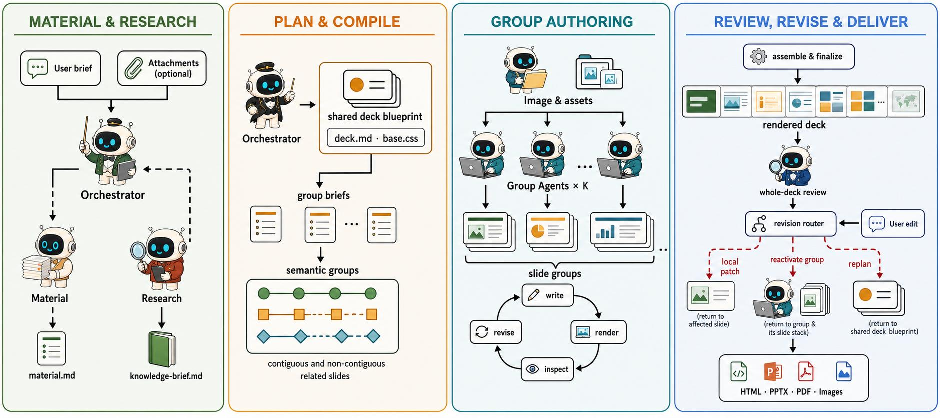
\includegraphics[width=0.90\textwidth]{figures/fig2_release_workflow.pdf}
\caption{\textbf{The full authoring and revision lifecycle in \sys{}.}
Material and Research ground inputs on demand; the Orchestrator writes the blueprint and group briefs; Image
prepares required bitmaps. Group Agents run parallel render--inspect--revise loops, whole-deck Review checks
cross-group relations, and the revision router replays the smallest responsible unit. Deterministic tools
transfer assets, render, validate, and package HTML, PPTX, PDF, and image delivery.}
\label{fig:release-workflow}
\end{figure*}


\subsection{Grouping, Visual Critique, and the Revision Loop}

\textbf{Dependency-aligned grouping.} MuralPresenter partitions the page set into complete, non-overlapping groups according to narrative, design, and asset affinity. Deck-level dependency closure decomposes into: \[
\mathrm{DC}(D)=\underbrace{\frac{1}{K}\!\!\sum_{k:\,\exists j,\,\{a_k\}\cup T_k\subseteq G_j}\!\!\mathbf{1}[\Phi_k\ \text{closed}]}_{\text{within-group: closed by one Group Agent}}
\;+\;
\underbrace{\frac{1}{K}\!\!\sum_{k:\,\nexists j,\,\{a_k\}\cup T_k\subseteq G_j}\!\!\mathbf{1}[\Phi_k\ \text{closed}]}_{\text{cross-group: backstopped by review}}.
\] The grouping goal is to pull as many strong dependencies as possible into the within-group term, leaving only a small number of cross-group relations to whole-deck review; we measure this gap in experiments (§6). Independent groups generate in parallel.

\textbf{Two-level visual critique.} Many defects surface only when rendered. MuralPresenter makes pixel inspection a first-class operation at two levels. Within a group, the Group Agent renders each page, revises until it holds in pixels, then reviews a group contact sheet for rhythm and repetition. At the deck level, Review inspects the full rendered deck in an isolated context; this independent-critic design also carries over to data synthesis (§4). Review is deliberately restrained: deterministic rendering imposes a hard gate only for CJK-font breakage; all other signals are returned as advice.

\textbf{Scope-based revision.} Post-generation edits reuse persistent state. Given an edit, the router conservatively infers an impact set \(I\): the directly touched pages plus any pages implicated through known cross-slide relations. Let the declared responsibility units be \(\mathcal{U} = \bigl\{\{i\} \mid i \in [N]\bigr\} \cup \{G_1,\ldots,G_m\} \cup \{[N]\}\), ordered by inclusion; the routing policy selects: \[
\mathrm{scope}(I) \;=\; \min_{U \in \mathcal{U}}\; U \quad \text{s.t.} \quad I \subseteq U.
\] This formalizes the implemented routing policy, not a learned optimizer: the system does not guarantee globally minimal cost or complete dependency knowledge, and escalates when impact is ambiguous. Concretely: a single-page patch goes through the Orchestrator; within-group relation changes reactivate the corresponding Group Agent \(\tau^{G_j}\); new facts or assets restart Research or Image on demand; structural changes (pages added, removed, reordered, or title chain altered) update the partition and trigger whole-deck review. Edit quality and preservation of untouched pages are tested in multi-turn experiments (§6). The final artifact is structured HTML, exportable to images, PDF, and PPTX.

\section{Long-Horizon Agentic Data Synthesis}

This section describes our data pipeline: task-dataset construction, trajectory synthesis with external verification, and multi-stage filtering (Figure~\ref{fig:data-synthesis}). We distinguish the controlled 9B corpus from the larger heterogeneous 27B training cohort.

\begin{figure}[H]
\centering
\begin{tikzpicture}
\node[inner sep=0] (datafig) {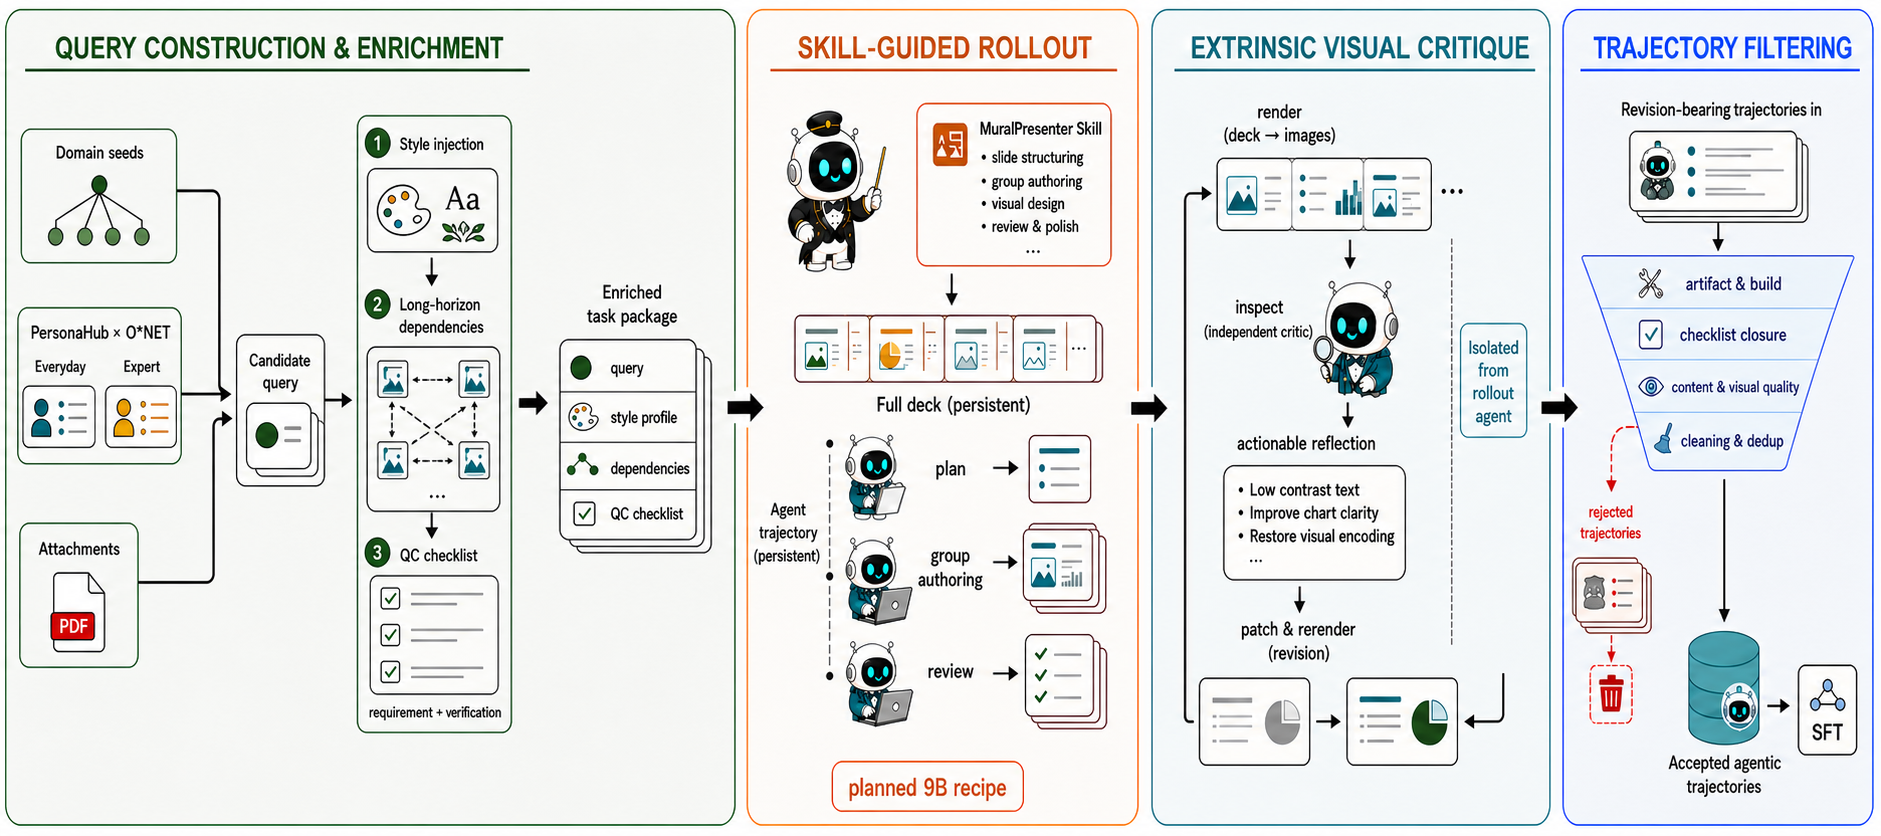
\includegraphics[width=\linewidth]{figures/fig3_long_horizon_agentic_data_synthesis.png}};
\node[fill=white,draw=auditorange,rounded corners=1.5pt,inner xsep=4pt,inner ysep=2pt,font=\scriptsize\sffamily,text=auditorange] at ($(datafig.south west)!0.493!(datafig.south east)+(0,0.43cm)$) {MuralPresenter-9B corpus};
\end{tikzpicture}
\caption{\textbf{Long-horizon agentic data synthesis.} Three query tracks feed a shared enrichment layer that injects a Style profile, constructs task-conditioned long-horizon dependencies, and compiles them into a checklist for downstream QC. A Skill-guided rollout preserves planning, group authoring, and review; an isolated visual critic induces render-grounded revisions; layered filtering retains only structurally complete trajectories that close the checklist. This controlled pipeline produces the MuralPresenter-9B corpus; the 27B cohort differs in teacher provenance and scale.}
\label{fig:data-synthesis}
\end{figure}

\subsection{Query Construction}

High-quality long-horizon training requires tasks whose structure is checkable across the deck. For MuralPresenter-9B, we construct candidate queries from three complementary tracks and then apply a shared enrichment layer. A Style profile sampled from a unified taxonomy is woven into the query as concrete guidance for color, typography, decorative motifs, and whitespace. The pipeline then constructs task-conditioned long-horizon dependencies, such as section quotas, narrative carry-over, cross-slide numeric consistency, motif continuity, loop closure, and explicit cross-slide references. We do not define long-horizon structure by a fixed number of constraints: each dependency records its type, concrete requirement, and closure condition. It is then compiled into a \texttt{longhorizon\_checklist} item specifying both the requirement and how downstream QC should verify it.

\textbf{Track 1: Domain-seed expansion.} From a hierarchical domain pool, seed topics expand into tasks spanning diverse disciplines and scenarios, emphasizing breadth and diversity.

\textbf{Track 2: Persona-driven real scenarios (PersonaHub \(\times\) O*NET).} Speaker personas are matched to tasks via the O*NET taxonomy in two tiers: a general everyday tier and an expert/elite tier with greater domain depth and longer dependency spans. From 84 initial pilot combinations, cleaning retained 82 across 65 occupations; 20 became end-to-end queries.

\textbf{Track 3: Attachment-driven reverse synthesis.} This track reverse-constructs attachment-bearing tasks from real documents, requiring the system to ground in, cite, and reorganize content.

After the three tracks merge, they share the same Style taxonomy, output schema, dependency representation, checklist compiler, and deduplication policy. The resulting task package contains the user-facing query, the injected Style profile, explicit long-horizon dependencies, and their QC checklist. Rollout and filtering therefore use the same dependency contract rather than reconstructing acceptance criteria after generation.

\subsection{Skill-Guided Trajectory Synthesis}

Given a task, a teacher model autonomously generates the full presentation under the MuralPresenter process described in §3, retaining planning, delegation, render inspection, diagnosis, patching, and re-rendering in the trajectory—making the supervision target an executable authoring process rather than merely the final HTML.

To avoid self-verification bias, we introduce external verification: an independent visual critic judges rendered artifacts in an isolated context, identifies pixel-only defects (overflow, broken images, low contrast), and returns actionable revisions that are injected back as feedback. The resulting trajectories thus carry reflective behavior grounded in real observation.

\textbf{Controlled 9B corpus.} To test whether the full workflow can be learned from a small, reproducibly specified corpus, we construct a controlled setting. DeepSeek-V4-Flash executes the authoring workflow as the rollout backbone, while Gemini-3.5-Flash provides render-conditioned visual critique. Deterministic validation and quality filtering retain exactly 1,000 post-QC training trajectories from \resulttbd{[TBD:9B\_TASKS]} tasks. We fine-tune Qwen-3.5-9B for \resulttbd{[TBD:9B\_EPOCH]} epochs with context length \resulttbd{[TBD:9B\_CTX]} on \resulttbd{[TBD:9B\_GPU]} GPUs, consuming \resulttbd{[TBD:9B\_GPUH]} GPU-hours.

\textbf{Heterogeneous 27B cohort.} MuralPresenter-27B is obtained by full-parameter supervised fine-tuning on quality-filtered agent trajectories generated predominantly by a higher-capability proprietary frontier teacher under the same authoring workflow. The trajectories retain planning, tool use, render inspection, diagnosis, revision, and re-rendering actions rather than only final HTML. The exact teacher identity is withheld because of commercial confidentiality constraints; we instead report the complete data-processing pipeline, corpus statistics, optimization settings, and compute below. The cohort draws from six heterogeneous historical batches. After QC-v2 filtering: 17,171 tasks and 304,275 valid trajectories; 16,073 tasks / 293,846 trajectories pass structural validation into the SFT candidate set; 293,436 base trajectories are retained after removing anomalous and incomplete samples. After Mixture-v2 resampling: 318,422 training exposures, 7.3127B content tokens, and 56,458 packed sequences. Gemini-3.5-Flash is used only for post-hoc quality scoring in this cohort, not as a rollout teacher or critic. This cohort does not share teacher provenance with the 9B corpus.

\subsection{Trajectory Filtering}

Multi-stage filtering ensures data quality: deterministic checks verify artifacts, page coverage, build success, and rendering; structural and constraint checks verify cross-slide requirements and user constraints item by item; quality scoring rates content and visual consistency; trajectory-level cleaning removes anomalous, incomplete, and near-duplicate samples. Failed or unverifiable trajectories are counted for statistics but never relabeled as usable data. We distinguish query, rollout, completion, and acceptance counts, report per-stage retention and rejection reasons in the data card, and summarize the post-filtering scale in §6.

% Generated mechanically from the reviewed Markdown source.
% Controller edits should be made in both source and LaTeX when material.

\section{ThreadBench}

\subsection{Process–Artifact Evaluation}

A polished deck can conceal a broken handoff: research evidence may never reach the plan, a planned image may never be used, or a rendered defect may never be repaired. Final-only scores see the artifact but cannot locate the broken transfer. ThreadBench therefore evaluates case-specific process evidence separately from the delivered deck. It is process-aware and artifact-grounded; it does not claim coverage of every engineering stage.

\begin{figure}[H]
\centering
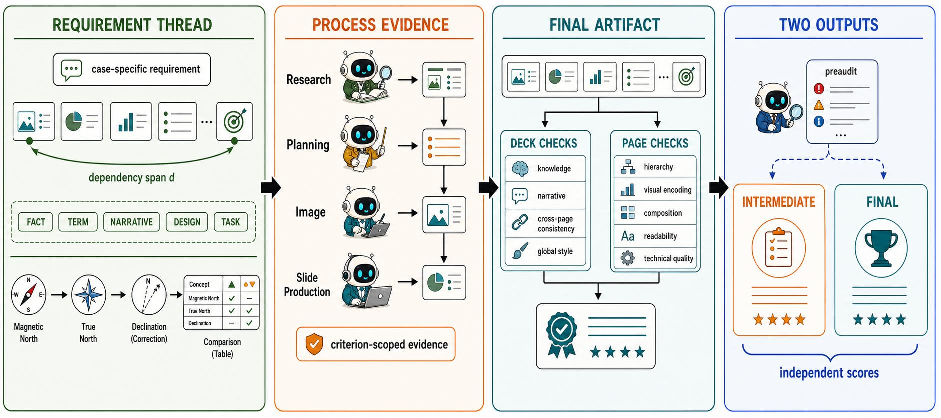
\includegraphics[width=\linewidth]{figures/fig4_threadbench_anatomy.pdf}
\caption{\textbf{Anatomy of ThreadBench.} A case-specific requirement defines an observable source-to-target closure rule across a deck. Intermediate evaluation follows anchored evidence through Research, Planning, Image, and Slide Production, whereas Final evaluation inspects the canonical rendered deck at deck and page granularity. The two layers produce independent scores rather than a single blended metric. The animal-navigation thread is the current formal reference case.}
\label{fig:threadbench-anatomy}
\end{figure}

\subsection{Requirement Threads and the Two-Layer Rubric}

Figure~\ref{fig:threadbench-anatomy} makes the evaluation unit explicit. A requirement thread starts from a source requirement or anchor, specifies a distant target and an observable closure rule, and may encode factual, terminological, narrative, design, or task-level dependence. The Intermediate layer evaluates seven criterion families across Research, Planning, Image, and Slide Production, using criterion-scoped packets that expose only relevant anchored evidence. The Final layer evaluates the canonical artifact in two groups: Deck combines a Knowledge checklist with six whole-deck dimensions, while Page scores five visual and technical dimensions for every canonical page. The complete criterion inventory and dimension definitions are in Appendix~\ref{app:protocol}.

\subsection{Scoring and Release Boundary}

The Judge first matches evidence to explicit anchors; code then derives 0/0.5/1 scores (Knowledge is binary). Deck and Page each receive one weakest-dimension decay, whereas Intermediate does not:

\[
G_{\mathrm{eff}}=G_{\mathrm{base}}[1-0.3(1-G_{\min})],\quad
F=\tfrac12(Deck_{\mathrm{eff}}+Page_{\mathrm{eff}}),\quad
I=\operatorname{mean}(R,P,I_m,S).
\]

where \(I_m\) denotes the Image dimension and only applicable Intermediate dimensions enter the mean. The released Intermediate \(I\) and Final \(F\) fields remain independent and are never collapsed into one scalar. The executable v004 contract currently specifies one formal reference case (\url{Education/Education-lh-Animal_navigation}). Appendix~\ref{app:protocol} gives the N/A semantics, major-defect deductions, optional non-scoring Preaudit, and human–Judge calibration; multi-domain expansion and explicit span diagnostics remain outside the current release.

\section{Experiments}

We organize experiments around four research questions. \textbf{RQ1 (general quality):} How good are the complete decks that MuralPresenter produces under general-quality evaluation? \textbf{RQ2 (multi-turn revision):} Without dedicated editing training, can it perform multi-turn edits? \textbf{RQ3 (process–artifact consistency):} Does the production chain preserve requirements and evidence through intermediate stages and into the final deck? \textbf{RQ4 (design choices):} How much do the delegation boundary, responsibility topology, two-level visual critique, and trajectory supervision each contribute?

\subsection{Setup}

\textbf{MuralPresenter-9B.} We use DeepSeek-V4-Flash as the rollout backbone and Gemini-3.5-Flash as the visual critic, sampling trajectories over \resulttbd{[TBD:9B\_TASKS]} training tasks (§4). Quality filtering retains exactly 1,000 post-QC trajectories. We fine-tune Qwen-3.5-9B with MS-SWIFT~\citep{zhao2024mswift} for \resulttbd{[TBD:9B\_EPOCH]} epochs, global batch 32, LR \(1\times10^{-5}\), and context length \resulttbd{[TBD:9B\_CTX]}, using \resulttbd{[TBD:9B\_GPU]} A800 GPUs for \resulttbd{[TBD:9B\_GPUH]} GPU-hours.

\textbf{Data and training (verified 27B).} MuralPresenter-27B uses the proprietary-teacher trajectory cohort described in §4: 293{,}436 base trajectories become 318{,}422 training exposures (\textasciitilde7.31B content tokens; \textasciitilde56{,}458 packed 128K sequences) after resampling and length filtering. We perform full-parameter SFT on Qwen-3.5-27B via the Megatron backend of MS-SWIFT: 128K context, 1 epoch, global batch 32, LR \(2\times10^{-5}\) with cosine decay to \(1\times10^{-6}\) after 5\% warmup, on 32 80GB GPUs (4 nodes, TP=4, CP=2, DP=4, micro-batch 1, gradient accumulation 8); the vision encoder and modality aligner are frozen. Training runs 1{,}764 steps in \textasciitilde50.3 hours (\textasciitilde1{,}604 GPU-hours). Gemini-3.5-Flash serves only as the QC-stage quality scorer. The full data/model ledger is in Appendix~\ref{app:protocol}.

\textbf{Baselines.} ThreadBench retains six strong general-purpose controls: Opus-4.7, Sonnet-5, GPT-5.6-luna, Gemini-3.5-Flash, Qwen-3.7-plus, and Kimi-k3. Existing-benchmark reruns use a compact five-system cohort: the 9B synthesis pipeline (DeepSeek-V4-Flash + Gemini-3.5-Flash), untuned Qwen-3.5-9B and Qwen-3.6-27B controls, and our 9B and 27B models. All five share the same benchmark inputs and adapter. To expose absolute position on each external benchmark, Tables~\ref{tab:general}--\ref{tab:edit} also include selected leading systems from the original papers in a separate \emph{reported} block. These values retain their source protocols, are not our reruns, and are never pooled with the unified cohort or entered into significance tests; complete reported tables appear in Appendix~\ref{app:protocol}.

\textbf{Interpretation boundary.} The 9B and 27B checkpoints differ in teacher provenance, corpus scale, base model, and training recipe. We report both as system variants but do not interpret their difference as a controlled scaling or data-efficiency result. We conduct RQ4 ablations in the 9B setting with the same 1K corpus and fixed training variables. Comparisons against proprietary frontier controls on ThreadBench are end-to-end system comparisons and do not establish teacher-independent generalization.

\textbf{Metric contracts.} PresentBench~\citep{chen2026presentbench} and SlidesGen-Bench~\citep{yang2026slidesgenbench} measure general quality, DECKBench~\citep{jang2026deckbench} measures multi-turn revision, and ThreadBench (§5) measures process–artifact consistency via separate Intermediate and Final scores with dimension-level diagnostics. Bounded quality, similarity, success, and ThreadBench scores are interpreted as higher-is-better; SlidesGen-Bench PEI remains an ordinal editability level, while signed DECKBench change metrics retain the official protocol's direction and are not merged with absolute quality scores. We freeze the official metric versions, direction, aggregation code, and hashes for all runs. Full dimensions and secondary diagnostics are in Appendix~\ref{app:protocol}.

\subsection{Main Results}

\textbf{General generation quality (RQ1).} Table~\ref{tab:general} places the five-system rerun cohort beside selected original-paper leaders on PresentBench Overall and SlidesGen-Bench Content, Aesthetics, and Editability (PEI). Full sub-dimensions and reported systems are in Appendix~\ref{app:protocol}. This table addresses general deck quality and draws no conclusion about long-horizon consistency.

\begin{table}[!htbp]
\centering
\small
\caption{RQ1: selected original-paper leaders (reported under source protocols) and our five-system unified reruns on PresentBench and SlidesGen-Bench. Full reported systems and dimensions are in Appendix~\ref{app:protocol}.}
\label{tab:general}
\begingroup
\let\texttt\resulttbd
\setlength{\tabcolsep}{4pt}
\begin{tabularx}{\linewidth}{@{}>{\raggedright\arraybackslash}Xcccc@{}}
\toprule
& PresentBench & \multicolumn{3}{c}{SlidesGen-Bench} \\
\cmidrule(lr){2-2}\cmidrule(lr){3-5}
System & Overall & Content & Aesthetics & Editability (PEI) \\
\midrule
\multicolumn{5}{l}{\emph{Original-paper references (reported)}} \\
NotebookLM       & 62.5 & 74.21 & 22.82 & L0 \\
Zhipu            & ---  & 88.29 & 22.06 & L2 \\
Skywork-Banana   & ---  & 83.83 & 27.28 & L1 \\
Quark            & ---  & 81.40 & 16.86 & L3 \\
\midrule
\multicolumn{5}{l}{\emph{Unified reruns (same inputs and adapter)}} \\
9B synth. pipeline (DS-V4 + Gemini-3.5) & \resulttbd{[TBD:G\_TC\_PB]} & \resulttbd{[TBD:G\_TC\_SGC]} & \resulttbd{[TBD:G\_TC\_SGA]} & \resulttbd{[TBD:G\_TC\_SGE]} \\
Qwen-3.5-9B (untuned)  & \resulttbd{[TBD:G\_Q9\_PB]}  & \resulttbd{[TBD:G\_Q9\_SGC]}  & \resulttbd{[TBD:G\_Q9\_SGA]}  & \resulttbd{[TBD:G\_Q9\_SGE]} \\
Qwen-3.6-27B (untuned) & \resulttbd{[TBD:G\_Q27\_PB]} & \resulttbd{[TBD:G\_Q27\_SGC]} & \resulttbd{[TBD:G\_Q27\_SGA]} & \resulttbd{[TBD:G\_Q27\_SGE]} \\
MuralPresenter-9B  & \resulttbd{[TBD:G\_M9\_PB]}  & \resulttbd{[TBD:G\_M9\_SGC]}  & \resulttbd{[TBD:G\_M9\_SGA]}  & \resulttbd{[TBD:G\_M9\_SGE]} \\
MuralPresenter-27B & \resulttbd{[TBD:G\_M27\_PB]} & \resulttbd{[TBD:G\_M27\_SGC]} & \resulttbd{[TBD:G\_M27\_SGA]} & \resulttbd{[TBD:G\_M27\_SGE]} \\
\bottomrule
\end{tabularx}
\endgroup
\end{table}

The reported block anchors the published frontier at 62.5 PresentBench Overall (NotebookLM), 88.29 Content (Zhipu), 27.28 Aesthetics (Skywork-Banana), and PEI L3 (Quark). MuralPresenter-9B reaches \resulttbd{[TBD:G\_M9\_PB]} PresentBench Overall and MuralPresenter-27B reaches \resulttbd{[TBD:G\_M27\_PB]}, compared with \resulttbd{[TBD:G\_BEST\_CONTROL\_PB]} for the strongest unified-rerun control. On SlidesGen-Bench, the two models obtain Content/Aesthetics/PEI triples of \resulttbd{[TBD:G\_M9\_TRIPLE]} and \resulttbd{[TBD:G\_M27\_TRIPLE]}. Relative to the reported frontier, \resulttbd{[TBD:G\_REPORTED\_COMPARISON]}; within the controlled rerun cohort, the results indicate \resulttbd{[TBD:G\_RQ1\_INTERPRETATION]}. Neither comparison is used to infer long-horizon consistency.

\textbf{Multi-turn revision (RQ2).} Table~\ref{tab:edit} places the same five rerun systems beside selected DECKBench configurations reporting Deck Fidelity, Layout Quality, Transition Similarity, \(\Delta\)-DTW, and \(\Delta\)-Transition Similarity. PPT-Eval~\citep{gandhi2026ppteval} remains a supplementary transfer test and includes its reported leading reference. Complete original-paper fields are in Appendix~\ref{app:protocol}. Transfer from inspect--diagnose--patch behavior is one hypothesis tested by RQ4.

\begin{table}[!htbp]
\centering
\footnotesize
\caption{RQ2: selected original-paper DECKBench references and our five-system unified reruns; PPT-Eval is supplementary and remains a separate protocol. Full reported fields are in Appendix~\ref{app:protocol}.}
\label{tab:edit}
\begingroup
\let\texttt\resulttbd
\setlength{\tabcolsep}{3pt}
\begin{tabularx}{\linewidth}{@{}>{\raggedright\arraybackslash}Xccccc@{}}
\toprule
& Deck & Slide & Deck & \multicolumn{2}{c}{Multi-turn} \\
\cmidrule(lr){2-2}\cmidrule(lr){3-3}\cmidrule(lr){4-4}\cmidrule(lr){5-6}
System & Fidelity & Layout Q. & Trans.\ Sim. & \(\Delta\)-DTW & \(\Delta\)-Trans.\ Sim. \\
\midrule
\multicolumn{6}{l}{\emph{Original-paper references (reported)}} \\
Auto-Slides (GPT-4o) & 0.591 & 0.998 & 0.858 & --- & --- \\
DECKBench (GPT-4o)   & 0.584 & 1.000 & 0.879 & --- & --- \\
GPT-5.1 sim. + GPT-5-mini edit. (High) & --- & --- & --- & 0.02278 & 0.03230 \\
Kimi K2 sim. + DeepSeek edit. (High)   & --- & --- & --- & 0.01549 & 0.04287 \\
\midrule
\multicolumn{6}{l}{\emph{Unified reruns (same inputs and adapter)}} \\
9B synth. pipeline (DS-V4 + Gemini-3.5) & \resulttbd{[TBD:E\_TC\_DFID]} & \resulttbd{[TBD:E\_TC\_SLQ]} & \resulttbd{[TBD:E\_TC\_DTSIM]} & \resulttbd{[TBD:E\_TC\_MDDTW]} & \resulttbd{[TBD:E\_TC\_MDTS]} \\
Qwen-3.5-9B (untuned)  & \resulttbd{[TBD:E\_Q9\_DFID]}  & \resulttbd{[TBD:E\_Q9\_SLQ]}  & \resulttbd{[TBD:E\_Q9\_DTSIM]}  & \resulttbd{[TBD:E\_Q9\_MDDTW]}  & \resulttbd{[TBD:E\_Q9\_MDTS]} \\
Qwen-3.6-27B (untuned) & \resulttbd{[TBD:E\_Q27\_DFID]} & \resulttbd{[TBD:E\_Q27\_SLQ]} & \resulttbd{[TBD:E\_Q27\_DTSIM]} & \resulttbd{[TBD:E\_Q27\_MDDTW]} & \resulttbd{[TBD:E\_Q27\_MDTS]} \\
MuralPresenter-9B  & \resulttbd{[TBD:E\_M9\_DFID]}  & \resulttbd{[TBD:E\_M9\_SLQ]}  & \resulttbd{[TBD:E\_M9\_DTSIM]}  & \resulttbd{[TBD:E\_M9\_MDDTW]}  & \resulttbd{[TBD:E\_M9\_MDTS]} \\
MuralPresenter-27B & \resulttbd{[TBD:E\_M27\_DFID]} & \resulttbd{[TBD:E\_M27\_SLQ]} & \resulttbd{[TBD:E\_M27\_DTSIM]} & \resulttbd{[TBD:E\_M27\_MDDTW]} & \resulttbd{[TBD:E\_M27\_MDTS]} \\
\midrule
\multicolumn{6}{l}{\emph{PPT-Eval (supplementary, official protocol, not comparable to the above)}} \\
& \multicolumn{2}{c}{Success Rate} & \multicolumn{3}{c}{Avg.\ Partial Score} \\
Claude-4.5-Opus (reported) & \multicolumn{2}{c}{45\%} & \multicolumn{3}{c}{57\%} \\
MuralPresenter-27B & \multicolumn{2}{c}{\resulttbd{[TBD:E\_M27\_PESR]}} & \multicolumn{3}{c}{\resulttbd{[TBD:E\_M27\_PEPS]}} \\
\bottomrule
\end{tabularx}
\endgroup
\end{table}

The reported DECKBench block exposes the published range without constructing a fictitious composite baseline: Auto-Slides leads the displayed Fidelity value, DECKBench (GPT-4o) leads Layout and Transition Similarity, and the two high-granularity simulator/editor configurations provide the multi-turn references. Across unified reruns, MuralPresenter-9B changes Deck Fidelity and Layout Quality by \resulttbd{[TBD:E\_M9\_SUMMARY]} relative to untuned Qwen-3.5-9B, while MuralPresenter-27B changes them by \resulttbd{[TBD:E\_M27\_SUMMARY]} relative to its 27B control. The multi-turn deltas show \resulttbd{[TBD:E\_MULTITURN\_INTERPRETATION]}; relative to reported external references, \resulttbd{[TBD:E\_REPORTED\_COMPARISON]}. PPT-Eval yields \resulttbd{[TBD:E\_PPTEVAL\_INTERPRETATION]} against the reported 45\%/57\% Claude-4.5-Opus reference. Together with RQ4, this supports \resulttbd{[TBD:E\_RQ2\_CONCLUSION]} about transfer from inspect--diagnose--patch supervision.

\textbf{Process–artifact consistency (RQ3).} Table~\ref{tab:thread} reports ThreadBench Intermediate and Final scores along with interpretable group breakdowns (Deck and Page effective scores). These are the two independent outputs of the v004 scoring contract (§5.3). Dimension-level diagnostics for all systems are in Appendix~\ref{app:protocol}.

\begin{table}[!htbp]
\centering
\small
\caption{RQ3: ThreadBench process–artifact consistency. Intermediate and Final are independent 0–1 scores; Deck and Page are the two Final sub-groups after weakest-dimension decay.}
\label{tab:thread}
\begingroup
\let\texttt\resulttbd
\setlength{\tabcolsep}{5pt}
\begin{tabularx}{\linewidth}{@{}>{\raggedright\arraybackslash}Xcccc@{}}
\toprule
& \multicolumn{1}{c}{Intermediate} & \multicolumn{3}{c}{Final} \\
\cmidrule(lr){2-2}\cmidrule(lr){3-5}
System & Score & Score & Deck\(_{eff}\) & Page\(_{eff}\) \\
\midrule
Opus-4.7            & \resulttbd{[TBD:T\_OP\_INT]}  & \resulttbd{[TBD:T\_OP\_FIN]}  & \resulttbd{[TBD:T\_OP\_DECK]} & \resulttbd{[TBD:T\_OP\_PAGE]} \\
Sonnet-5            & \resulttbd{[TBD:T\_SN\_INT]}  & \resulttbd{[TBD:T\_SN\_FIN]}  & \resulttbd{[TBD:T\_SN\_DECK]} & \resulttbd{[TBD:T\_SN\_PAGE]} \\
GPT-5.6-luna        & \resulttbd{[TBD:T\_LU\_INT]}  & \resulttbd{[TBD:T\_LU\_FIN]}  & \resulttbd{[TBD:T\_LU\_DECK]} & \resulttbd{[TBD:T\_LU\_PAGE]} \\
Gemini-3.5-Flash    & \resulttbd{[TBD:T\_GM\_INT]}  & \resulttbd{[TBD:T\_GM\_FIN]}  & \resulttbd{[TBD:T\_GM\_DECK]} & \resulttbd{[TBD:T\_GM\_PAGE]} \\
Qwen-3.7-plus       & \resulttbd{[TBD:T\_QW\_INT]}  & \resulttbd{[TBD:T\_QW\_FIN]}  & \resulttbd{[TBD:T\_QW\_DECK]} & \resulttbd{[TBD:T\_QW\_PAGE]} \\
Kimi-k3             & \resulttbd{[TBD:T\_KM\_INT]}  & \resulttbd{[TBD:T\_KM\_FIN]}  & \resulttbd{[TBD:T\_KM\_DECK]} & \resulttbd{[TBD:T\_KM\_PAGE]} \\
\midrule
MuralPresenter-9B  & \resulttbd{[TBD:T\_M9\_INT]}  & \resulttbd{[TBD:T\_M9\_FIN]}  & \resulttbd{[TBD:T\_M9\_DECK]} & \resulttbd{[TBD:T\_M9\_PAGE]} \\
MuralPresenter-27B & \resulttbd{[TBD:T\_M27\_INT]} & \resulttbd{[TBD:T\_M27\_FIN]} & \resulttbd{[TBD:T\_M27\_DECK]} & \resulttbd{[TBD:T\_M27\_PAGE]} \\
\bottomrule
\end{tabularx}
\endgroup
\end{table}

MuralPresenter-9B obtains \resulttbd{[TBD:T\_M9\_INT]}/\resulttbd{[TBD:T\_M9\_FIN]} Intermediate/Final, and MuralPresenter-27B obtains \resulttbd{[TBD:T\_M27\_INT]}/\resulttbd{[TBD:T\_M27\_FIN]}. Relative to the strongest general-purpose baseline, the corresponding differences are \resulttbd{[TBD:T\_M9\_DELTA]} and \resulttbd{[TBD:T\_M27\_DELTA]}. The Deck/Page split reveals \resulttbd{[TBD:T\_RQ3\_INTERPRETATION]}, showing whether the dominant bottleneck lies in requirement transfer or rendered-page quality.

\subsection{Ablation (RQ4)}

Table~\ref{tab:ablation} reports four one-factor-at-a-time ablations against one shared Full reference in the 9B setting, using the same 1K training corpus and holding all other training variables fixed. \textbf{Delegation boundary:} single-context or always-delegate. \textbf{Responsibility topology:} per-slide or fixed-adjacent grouping; this isolates whether dependency-aligned grouping contributes beyond generic decomposition. \textbf{Two-level visual critique:} removing group-level or whole-deck review individually. \textbf{Trajectory supervision:} output-only SFT or removing inspect--diagnose--patch steps. Primary scores are ThreadBench Intermediate and Final; the cross-page semantic-consistency dimension provides a topology-sensitive diagnostic.

\begin{table}[!htbp]
\centering
\footnotesize
\caption{RQ4 controlled ablations against one shared Full reference. Intermediate and Final are aggregate outputs; Cross-page is the Final Deck semantic-consistency dimension.}
\label{tab:ablation}
\begingroup
\let\texttt\resulttbd
\setlength{\tabcolsep}{3pt}
\begin{tabularx}{\linewidth}{@{}>{\raggedright\arraybackslash}p{0.19\linewidth}>{\raggedright\arraybackslash}Xccc@{}}
\toprule
Factor & Variant & Intermediate & Final & Cross-page \\
\midrule
Full reference (ours) & on-demand + dep.-aligned + both critique + full traj. & \resulttbd{[TBD:A\_FULL\_INT]} & \resulttbd{[TBD:A\_FULL\_FIN]} & \resulttbd{[TBD:A\_FULL\_XSEM]} \\
\midrule
Delegation boundary & Single-context      & \resulttbd{[TBD:A\_DEL\_SC\_INT]}  & \resulttbd{[TBD:A\_DEL\_SC\_FIN]} & \resulttbd{[TBD:A\_DEL\_SC\_XSEM]} \\
                    & Always-delegate     & \resulttbd{[TBD:A\_DEL\_AD\_INT]}  & \resulttbd{[TBD:A\_DEL\_AD\_FIN]} & \resulttbd{[TBD:A\_DEL\_AD\_XSEM]} \\
\midrule
Responsibility topology & Per-slide ownership & \resulttbd{[TBD:A\_TOP\_PS\_INT]}  & \resulttbd{[TBD:A\_TOP\_PS\_FIN]} & \resulttbd{[TBD:A\_TOP\_PS\_XSEM]} \\
                    & Fixed-adjacent      & \resulttbd{[TBD:A\_TOP\_FA\_INT]}  & \resulttbd{[TBD:A\_TOP\_FA\_FIN]} & \resulttbd{[TBD:A\_TOP\_FA\_XSEM]} \\
\midrule
Two-level visual critique & w/o group-level     & \resulttbd{[TBD:A\_VIS\_NG\_INT]}  & \resulttbd{[TBD:A\_VIS\_NG\_FIN]} & \resulttbd{[TBD:A\_VIS\_NG\_XSEM]} \\
                    & w/o whole-deck      & \resulttbd{[TBD:A\_VIS\_NW\_INT]}  & \resulttbd{[TBD:A\_VIS\_NW\_FIN]} & \resulttbd{[TBD:A\_VIS\_NW\_XSEM]} \\
\midrule
Trajectory supervision & Output-only SFT     & \resulttbd{[TBD:A\_SUP\_OO\_INT]}  & \resulttbd{[TBD:A\_SUP\_OO\_FIN]} & \resulttbd{[TBD:A\_SUP\_OO\_XSEM]} \\
                    & w/o inspect--patch  & \resulttbd{[TBD:A\_SUP\_NI\_INT]}  & \resulttbd{[TBD:A\_SUP\_NI\_FIN]} & \resulttbd{[TBD:A\_SUP\_NI\_XSEM]} \\
\bottomrule
\end{tabularx}
\endgroup
\end{table}

Replacing dependency-aligned groups with per-slide or fixed-adjacent ownership changes Cross-page consistency by \resulttbd{[TBD:A\_TOPOLOGY\_EFFECT]}; changing the delegation boundary changes Final by \resulttbd{[TBD:A\_DELEGATION\_EFFECT]}. Removing group- or deck-level critique yields \resulttbd{[TBD:A\_CRITIQUE\_EFFECT]}, while output-only and no-inspect supervision yield \resulttbd{[TBD:A\_SUPERVISION\_EFFECT]}. The combined pattern yields \resulttbd{[TBD:A\_RQ4\_INTERPRETATION]}, separating the responsibility-topology effect from generic multi-Agent decomposition.

% Generated mechanically from the reviewed Markdown source.
% Controller edits should be made in both source and LaTeX when material.

\section{Case Study: Tracing an Animal-Navigation Deck}

The formal ThreadBench reference case asks for a science-teaching deck on animal navigation, coupling geomagnetic, solar, and stellar compasses with mechanism explanations, scientific diagrams, real images, and an exact six-column-by-three-row comparison table. This creates one long-range thread: evidence established during research must survive page planning and mechanism exposition, then reappear under a consistent comparison schema. Research records the evidence and terminology; the Orchestrator maps each requirement to deck and page contracts plus image tasks; Group Agents jointly author related mechanism and synthesis pages; and whole-deck Review checks the closing comparison against the concepts introduced earlier. The persistent artifacts expose three inspectable handoffs: evidence to plan, plan and assets to pages, and page groups to the assembled deck.

The case-specific rubric then localizes failures that look similar in the final artifact: missing mechanism evidence belongs to Research, grounded facts dropped from page contracts to Planning, and unused assets or uninspected renders to production; incorrect comparison dimensions, inconsistent terminology, and unreadable encodings remain final-deck failures even when intermediate artifacts exist. This separation gives practitioners a concrete repair target and prevents process completion from substituting for artifact quality. We use the case as a qualitative trace, while the controlled 9B ablations provide the causal test of responsibility topology. The evidence boundary remains narrow: 9B and 27B differ in data and training, LLM judgments remain bounded by their measured human agreement, the benchmark currently has one formal case, and HTML-to-PDF/PPTX conversion does not test speech, rehearsal, animation, or native-office editing. The case therefore supports failure localization, not broad domain-generalization claims.

\section{Conclusion}

Long-horizon presentation authoring fails when decisions that persist across pages outlive the context or owner responsible for them. MuralPresenter addresses this mismatch by externalizing deck state, assigning dependent pages to shared Group Agents, and combining group-level pixel inspection with independent whole-deck review. We train MuralPresenter-9B on 1,000 quality-controlled trajectories and MuralPresenter-27B on a larger heterogeneous cohort, with both systems preserving planning, diagnosis, and repair supervision. Across PresentBench, SlidesGen-Bench, and DECKBench, the models achieve \resulttbd{[TBD:CONC\_GENERAL]}; on ThreadBench, they achieve \resulttbd{[TBD:CONC\_THREAD]}. Controlled 9B ablations show \resulttbd{[TBD:CONC\_ABLATION]}, clarifying the roles of responsibility topology, delegation, visual critique, and trajectory supervision. The animal-navigation case further traces one requirement from evidence through planning and assets into rendered pages. Limitations remain: the two model sizes are not a controlled scaling comparison, ThreadBench currently contains one formal case, and HTML-to-PDF/PPTX conversion does not evaluate rehearsal, animation, or native-office editing. Within these boundaries, the results establish MuralPresenter as an auditable framework for studying and improving long-horizon presentation consistency.

\label{main:end}

\bibliographystyle{iclr2026_conference}
\bibliography{references}

\appendix
\section{Evaluation Protocol and Reproducibility Details}
\label{app:protocol}
\setcounter{figure}{0}
\renewcommand{\thefigure}{A\arabic{figure}}
\renewcommand{\theHfigure}{A\arabic{figure}}

This appendix provides the full protocol, statistical conventions, complete official-benchmark dimension tables, a data/model contrast between MuralPresenter-9B and MuralPresenter-27B, and the reproducibility ledger.

\subsection{External-Baseline Protocol vs.\ Ablation Controls}

ThreadBench uses six general-purpose controls. Existing-benchmark reruns use the five-system cohort in Tables~\ref{tab:general}--\ref{tab:edit}: the 9B synthesis pipeline, two untuned controls, and two MuralPresenter models. Within each benchmark, reruns fix nominal inputs, Skill, renderer, adapter, and budget. The main tables promote selected original-paper leaders into a separate \emph{reported} block; the complete reported lists appear below. These values retain their source protocols and are never pooled with our reruns. Single-factor ablations (\S6.3) additionally hold backbone and training variables fixed; none of these descriptive comparisons is itself causal.

The current release contains one formal reference case and therefore does not support task-level confidence intervals or significance tests. Controlled ablations fix temperature, inputs, renderer, budget, and failure rules and use 3 seeds per variant; we report seed-level variation descriptively rather than treating it as task-level uncertainty. Missing artifacts, failures, and timeouts remain in the denominator; N/A and scored coverage are reported separately. External baselines, which differ in backbone, are references only and do not enter significance tests. We calibrate the LLM Judge against \resulttbd{[TBD:JUDGE\_N]} human-scored units from \resulttbd{[TBD:JUDGE\_CASES]} tasks, obtaining \resulttbd{[TBD:JUDGE\_AGREEMENT]} agreement under the protocol below.

\subsection{Original-Paper Reference Scores}

These are published aggregate values for context, not reproduced results or inputs to our hypothesis tests.

\paragraph{PresentBench (reported).} Overall scores from the original paper~\citep{chen2026presentbench} are shown below for direct visual comparison with our reruns.
\begin{center}\small
\begin{tabular}{lrlr}
\toprule System & Overall & System & Overall \\
\midrule
NotebookLM & 62.5 & Manus 1.6 & 57.8 \\
Tiangong & 54.7 & Zhipu & 53.6 \\
PPTAgent v2 & 50.2 & Gamma & 49.2 \\
Doubao & 48.0 & Qwen & 35.9 \\
\bottomrule
\end{tabular}
\end{center}

\paragraph{SlidesGen-Bench (reported).} Official Content/Aesthetics/PEI values~\citep{yang2026slidesgenbench}.
\begin{center}\small
\begin{tabular}{lccc}
\toprule System & Content (\%) & Aesthetics & PEI \\
\midrule
Zhipu & 88.29 & 22.06 & L2 \\
Kimi-Banana & 87.09 & 26.58 & L1 \\
Skywork-Banana & 83.83 & 27.28 & L1 \\
Kimi-Smart & 82.07 & 18.30 & L2 \\
Quark & 81.40 & 16.86 & L3 \\
Skywork & 81.29 & 20.69 & L2 \\
Kimi-Standard & 79.92 & 19.25 & L2 \\
NotebookLM & 74.21 & 22.82 & L0 \\
Gamma & 70.32 & 17.09 & L2 \\
\bottomrule
\end{tabular}
\end{center}

\paragraph{DECKBench (reported).} Task-1 values join the official slide- and deck-metric rows for the same
system/model; Task-2 retains the original simulator/editor configurations~\citep{jang2026deckbench}.
\begin{center}\small
\begin{tabular}{llccc}
\toprule System & Model & Deck Fidelity & Slide Layout & Deck TransSim \\
\midrule
Evo-Present & GPT-4o & 0.528 & 0.696 & 0.819 \\
SlideGen & GPT-4o & 0.566 & 0.960 & 0.856 \\
Auto-Slides & GPT-4o & 0.591 & 0.998 & 0.858 \\
DECKBench & GPT-4o & 0.584 & 1.000 & 0.879 \\
DECKBench & Qwen & 0.588 & 0.999 & 0.875 \\
\bottomrule
\end{tabular}
\end{center}
\begin{center}\small
\begin{tabular}{llccc}
\toprule User simulator & Editor & Granularity & $\Delta$DTW & $\Delta$TransSim \\
\midrule
GPT-5.1 & GPT-5-mini & Low & 0.01006 & 0.01594 \\
GPT-5.1 & GPT-5-mini & Medium & 0.01682 & 0.02145 \\
GPT-5.1 & GPT-5-mini & High & 0.02278 & 0.03230 \\
Kimi K2 & DeepSeek & Low & 0.01101 & -0.00147 \\
Kimi K2 & DeepSeek & Medium & 0.00249 & 0.00615 \\
Kimi K2 & DeepSeek & High & 0.01549 & 0.04287 \\
\bottomrule
\end{tabular}
\end{center}

\paragraph{PPT-Eval (reported).} Claude-4.5-Opus reaches 45\% Success Rate and 57\% Average Partial
Score in the official computer-use protocol~\citep{gandhi2026ppteval}; this is not directly comparable
to DECKBench or our HTML authoring runs.

\subsection{Full Dimensions of the Official Metrics}

\paragraph{PresentBench five dimensions.} The main table already gives Overall; here we add only the remaining five dimensions and do not repeat Overall.

\begin{center}
\small
\begingroup
\let\texttt\resulttbd
\setlength{\tabcolsep}{5pt}
\begin{tabularx}{\linewidth}{@{}>{\raggedright\arraybackslash}Xccccc@{}}
\toprule
System & Fund. & Vis.\&Lay. & Compl. & Corr. & Fidelity \\
\midrule
9B synth.\ pipeline & \resulttbd{[TBD:P5\_TC\_FU]} & \resulttbd{[TBD:P5\_TC\_VL]} & \resulttbd{[TBD:P5\_TC\_CP]} & \resulttbd{[TBD:P5\_TC\_CR]} & \resulttbd{[TBD:P5\_TC\_FI]} \\
Qwen-3.5-9B untuned & \resulttbd{[TBD:P5\_Q9\_FU]} & \resulttbd{[TBD:P5\_Q9\_VL]} & \resulttbd{[TBD:P5\_Q9\_CP]} & \resulttbd{[TBD:P5\_Q9\_CR]} & \resulttbd{[TBD:P5\_Q9\_FI]} \\
Qwen-3.6-27B untuned & \resulttbd{[TBD:P5\_Q27\_FU]} & \resulttbd{[TBD:P5\_Q27\_VL]} & \resulttbd{[TBD:P5\_Q27\_CP]} & \resulttbd{[TBD:P5\_Q27\_CR]} & \resulttbd{[TBD:P5\_Q27\_FI]} \\
MuralPresenter-9B  & \resulttbd{[TBD:P5\_M9\_FU]}  & \resulttbd{[TBD:P5\_M9\_VL]}  & \resulttbd{[TBD:P5\_M9\_CP]}  & \resulttbd{[TBD:P5\_M9\_CR]}  & \resulttbd{[TBD:P5\_M9\_FI]} \\
MuralPresenter-27B & \resulttbd{[TBD:P5\_M27\_FU]} & \resulttbd{[TBD:P5\_M27\_VL]} & \resulttbd{[TBD:P5\_M27\_CP]} & \resulttbd{[TBD:P5\_M27\_CR]} & \resulttbd{[TBD:P5\_M27\_FI]} \\
\bottomrule
\end{tabularx}
\endgroup
\end{center}

\paragraph{DECKBench full official fields.} The main table gives selected fields (deck Fidelity, slide Layout Quality, deck Transition Similarity, multi-turn \(\Delta\)-DTW and \(\Delta\)-Transition Similarity); here we complete the remaining official fields so that the union of main table and appendix covers every official DECKBench metric. Slide-level and deck-level PPL and Faithfulness are distinguished by distinct IDs. Systems match the main table.

\begin{center}
\footnotesize
\begingroup
\let\texttt\resulttbd
\setlength{\tabcolsep}{3pt}
\begin{tabularx}{\linewidth}{@{}>{\raggedright\arraybackslash}Xccccccc@{}}
\toprule
& \multicolumn{4}{c}{Slide-level} & \multicolumn{3}{c}{Deck-level} \\
\cmidrule(lr){2-5}\cmidrule(lr){6-8}
System & PPL & Faith. & Text Sim. & Fig.\ Sim. & PPL & Faith. & DTW \\
\midrule
9B synth.\ pipeline & \resulttbd{[TBD:E\_TC\_SPPL]} & \resulttbd{[TBD:E\_TC\_SFA]} & \resulttbd{[TBD:E\_TC\_STX]} & \resulttbd{[TBD:E\_TC\_SFG]} & \resulttbd{[TBD:E\_TC\_DPPL]} & \resulttbd{[TBD:E\_TC\_DFA]} & \resulttbd{[TBD:E\_TC\_DDTW]} \\
Qwen-3.5-9B untuned & \resulttbd{[TBD:E\_Q9\_SPPL]} & \resulttbd{[TBD:E\_Q9\_SFA]} & \resulttbd{[TBD:E\_Q9\_STX]} & \resulttbd{[TBD:E\_Q9\_SFG]} & \resulttbd{[TBD:E\_Q9\_DPPL]} & \resulttbd{[TBD:E\_Q9\_DFA]} & \resulttbd{[TBD:E\_Q9\_DDTW]} \\
Qwen-3.6-27B untuned & \resulttbd{[TBD:E\_Q27\_SPPL]} & \resulttbd{[TBD:E\_Q27\_SFA]} & \resulttbd{[TBD:E\_Q27\_STX]} & \resulttbd{[TBD:E\_Q27\_SFG]} & \resulttbd{[TBD:E\_Q27\_DPPL]} & \resulttbd{[TBD:E\_Q27\_DFA]} & \resulttbd{[TBD:E\_Q27\_DDTW]} \\
MuralPresenter-9B  & \resulttbd{[TBD:E\_M9\_SPPL]}  & \resulttbd{[TBD:E\_M9\_SFA]}  & \resulttbd{[TBD:E\_M9\_STX]}  & \resulttbd{[TBD:E\_M9\_SFG]}  & \resulttbd{[TBD:E\_M9\_DPPL]}  & \resulttbd{[TBD:E\_M9\_DFA]}  & \resulttbd{[TBD:E\_M9\_DDTW]} \\
MuralPresenter-27B & \resulttbd{[TBD:E\_M27\_SPPL]} & \resulttbd{[TBD:E\_M27\_SFA]} & \resulttbd{[TBD:E\_M27\_STX]} & \resulttbd{[TBD:E\_M27\_SFG]} & \resulttbd{[TBD:E\_M27\_DPPL]} & \resulttbd{[TBD:E\_M27\_DFA]} & \resulttbd{[TBD:E\_M27\_DDTW]} \\
\bottomrule
\end{tabularx}
\endgroup
\end{center}

\paragraph{ThreadBench dimension contract.} Table~\ref{tab:thread} reports the two official aggregates and the two effective Final group scores. Every run additionally retains the following dimension scores in \texttt{score\_result.json}; these are diagnostics, not a third aggregate.

\begin{center}\small
\begin{tabular}{lp{0.75\linewidth}}
\toprule Group & Dimensions \\
\midrule
Intermediate & Material/Research; Deck Planning; Image Asset Preparation; Slide Production and Local Verification \\
Final Deck & Knowledge; Audience/Goal Fit; Content Selection/Density; Narrative/Transitions; Pacing/Redundancy; Cross-page Semantic Consistency; Global Visual Consistency \\
Final Page & Information Hierarchy/Density; Text--Image Relationship/Visual Encoding; Composition/Alignment/Whitespace; Typography/Color/Readability; Technical Completeness/Asset Quality \\
\bottomrule
\end{tabular}
\end{center}

\paragraph{Intermediate criteria and scoring mechanics.} The compact main-text account omits the
criterion-level inventory shown below. Each criterion expands into topic-, requirement-, image-task-,
or page-specific units; the Judge receives only the anchors and evidence relevant to that unit.

\begin{center}\small
\begin{tabularx}{\linewidth}{@{}p{0.18\linewidth}p{0.15\linewidth}X@{}}
\toprule Dimension & Criteria & Evidence tested \\
\midrule
Material/Research & R01, R02 & Evidence coverage, source verification, conflict handling, and transfer into planning \\
Deck Planning & P01, P02 & Hard-requirement mapping, narrative structure, and per-page task specification \\
Image Preparation & I01, I02 & Task definition, acquisition strategy, inspection, selection, and page-level usage \\
Slide Production & S01 & Real rendering, defect detection, repair, and re-render confirmation \\
\bottomrule
\end{tabularx}
\end{center}

The Judge matches evidence to explicit anchors before deterministic code derives 0/0.5/1 atomic
scores; Knowledge is binary. N/A means semantically inapplicable and cannot substitute for a missing
required artifact. Atomic scores average into criteria and dimensions. Under v004, a major unit scored
0.5 or 0 deducts 0.1 or 0.2, respectively, from its dimension, with total deductions capped at 0.5 per
dimension. Deck and Page each receive the weakest-dimension decay defined in \S5, while Intermediate
does not. Optional Preaudit is non-scoring and passes only criterion-relevant defects to the formal
Judge. The released fields \texttt{intermediate\_case\_specific} and
\texttt{final\_output\_case\_specific} remain separate outputs.

\subsection{MuralPresenter-9B vs.\ MuralPresenter-27B Data/Model Ledger}

The table separates the evidence boundaries of the two sources. The 9B uses the controlled three-track synthesis pipeline and a 1K post-QC corpus; the 27B uses six heterogeneous historical batches at substantially larger scale. For the 27B, trajectories were generated predominantly by a higher-capability proprietary frontier teacher; the exact identity is withheld for commercial confidentiality reasons.

\begin{center}
\small
\begingroup
\let\texttt\resulttbd
\setlength{\tabcolsep}{4pt}
\begin{tabularx}{\linewidth}{@{}p{0.20\linewidth}XX@{}}
\toprule
Item & MuralPresenter-9B & MuralPresenter-27B \\
\midrule
Data source & controllable three-track synthesis (\S4) & six heterogeneous historical batches \\
Tasks & \resulttbd{[TBD:9B\_TASKS]} & 17{,}171 \\
Valid trajectories & --- & 304{,}275 \\
SFT candidate tasks & --- & 16{,}073 (93.6\%) \\
Base training trajectories & 1{,}000 (post-QC) & 293{,}436 \\
Training exposures & \resulttbd{[TBD:9B\_EXPOSURES]} & 318{,}422 \\
Rollout backbone & DeepSeek-V4-Flash & higher-capability proprietary frontier teacher (identity withheld) \\
Visual critic / QC & Gemini-3.5-Flash & Gemini-3.5 as QC scorer only \\
Base model & Qwen-3.5-9B & Qwen-3.5-27B \\
GPU-hours & \resulttbd{[TBD:9B\_GPUH]} & about 1{,}604 \\
Status & trained & trained \\
\bottomrule
\end{tabularx}
\endgroup
\end{center}

Here ``training exposures'' denotes samples entering optimization after filtering and length packing, a different quantity from ``base training trajectories''; if the 9B does no resampling/length packing, this entry is ---.

\subsection{Reproducibility Ledger}

For all reported runs, we freeze and record candidate systems and versions, benchmark/material hashes, renderer and model settings, inference budget and concurrency, Judge prompt and rubric, human-annotation protocol, and every criterion-, dimension-, group-, and case-level result. The current public contract specifies one formal case, which limits domain-level inference despite completed human--Judge calibration. The PersonaHub \(\times\) O*NET track is part of the frozen 9B construction corpus. Operational accounting (wall-clock, calls, tokens, estimated cost, context overlap, renders, concurrency) supports reproducibility but does not replace the separate Intermediate and Final scores or their dimension traces.

\paragraph{Run profile and trajectory-capture boundary.} The harness separates delivery-oriented inference from training-data synthesis. In inference mode, the model-facing working history may compact stale text and tool outputs and release consumed image payloads; exact tool results and the immutable execution Trace remain persisted for audit. In synthesis mode, history compaction and image dropping are disabled so that the context actually observed by the model matches the exported trajectory. An exact-raw recorder additionally stores the final provider request body, response bytes before SDK parsing, retry attempts, provider-exposed auxiliary vision traces, and content-addressed image evidence. A per-Agent integrity precheck gates conversion and rejects incomplete call--asset--response chains. This is an implementation and data-governance boundary, not a claimed algorithmic contribution; ``raw'' covers only provider-visible traffic and persisted artifacts, not hidden provider state.


\end{document}
